%\begin{tcolorbox}[title=TODO]
%Measurement results / analysis / discussion: 1/3
%\begin{itemize}
%\item whatever you have done, you must comment it, compare it to other systems, evaluate it
%\item usually, adequate graphs help to show the benefits of your approach
%\item caution: each result/graph must be discussed! what's the reason for this peak or why have you ovserved this effect
%\end{itemize}
%\end{tcolorbox}

\section{Image Size}
We were able to create a minimal \ac{OS} image with the Azure IoT Edge runtime
using \textit{reUpNix}. To achieve this, we created \textit{Nix} derivations
and modules for the \textit{Azure IoT Edge} runtime and the \textit{Azure IoT Edge
Identity Service}. We also created a \textit{Nix} derivation for the \ac{ADU} Agent.
Microsoft has the source code for the previously mentioned components
publicly available on GitHub, so we could build the \textit{Nix} packages directly
from source, which is written in Rust and C and uses Cargo and CMake respectively.
Further, we had to add the already existing \textit{Nix} package for \textit{Docker}
to the system configuration. Finally, since \textit{reUpNix} removes some unnecessary
Kernel modules, we had to add Kernel modules back to the system configuration in order
to be able to run \textit{Docker}. Most notably, we had to add the modules
\textit{br\_netfilter}, \textit{xt\_nat} and \textit{8021q} to the system configuration,
since they are required for \textit{Docker} networking.

We compared \textit{reUpNix}, \textit{NixOS 23.01}, \textit{Ubuntu 22.04}, and
\textit{Yocto Kirkstone} by their installed image size, with the methodology introduced
in chapter \ref{sec:image-size}. All system images feature an \ac{OCI}-compliant container runtime
and the Azure IoT Edge runtime. The results of the comparison are shown in table \ref{tab:image-size}.

\begin{table}[H]
	\centering
	\begin{tabular}{l|l|l}
	\toprule
		Operating System & Image Variation 1 & $\Delta$ Ubuntu\\
	\midrule
    \textbf{reUpNix} & \text{1 289 MB} & \color{ba-green}{- 1 010 MB} \\
    \textbf{NixOS 23.01} & \text{2 361 MB} & \textcolor{ba-red}{+ 62 MB} \\
    \textbf{Ubuntu 22.04} & \text{2 299 MB} & \text{-} \\
    \textbf{Yocto Kirkstone} & \text{4 933 MB} & \textcolor{ba-red}{+ 2 634 MB} \\
	\bottomrule
	\end{tabular}
	\caption{Image size by OS for each variation}
	\label{tab:image-size}
\end{table}
\noindent
We can see from table \ref{tab:image-size} that with its 1,289 Megabytes
\textit{reUpNix} has a 43\% smaller base image size than Microsoft's recommended
\textit{Ubuntu 22.04}. It is also 45\% smaller than the base image size of
\textit{NixOS 23.01}, which shows that the minification process is very effective
in minimizing the size of the \ac{OS} on disk despite having a fully working
Azure IoT Edge runtime installed.
To further illustrate the differences in size, refer to figure \ref{fig:image-size}.


\begin{figure}[htbp]
  \centering
  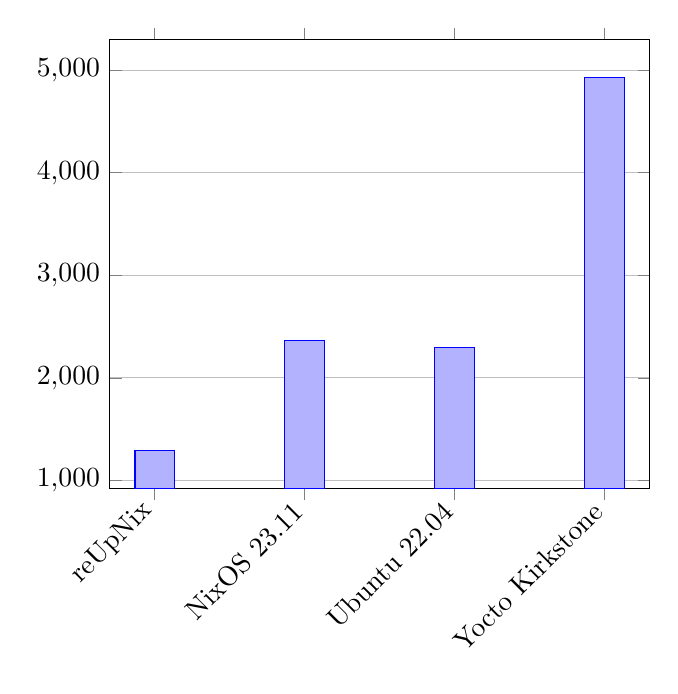
\begin{tikzpicture}
    \begin{axis}[
      ybar,
      bar width=0.5cm,
      % width=0.5\textwidth,
      % height=0.5\textwidth,
      xtick=data,
      xticklabels={
        {reUpNix},
        {NixOS 23.11},
        {Ubuntu 22.04},
        {Yocto Kirkstone}
      },
      x tick label style={rotate=45,anchor=east}, % Rotating labels
      ymajorgrids=true, % Major grid lines for y-axis
      ytick={0,1000,2000,3000,4000,5000}, % Y-axis tick marks
      extra y ticks={1000,2000,3000,4000}, % Additional y-axis tick marks
      extra y tick labels={}, % Remove labels for the extra ticks
      ]

      \addplot coordinates {
        (1,1289)
        (2,2361)
        (3,2299)
        (4,4933)
      };

    \end{axis}
  \end{tikzpicture}
\caption{Image size by OS in Megabytes}
\label{fig:image-size}
\end{figure}

\noindent
In contrary, the difference in image size between \textit{Ubuntu 22.04} and
\textit{NixOS} is only 62 Megabytes, which is unsurprising, since both are
general purpose \textit{Linux} distributions and not specifically designed
for embedded and \ac{IoT} systems. The largest image in this comparison is
\textit{Yocto Kirkstone}, which is 2,634 Megabytes larger than \textit{Ubuntu 22.04}.
However, it features no effort to minimize the size of the \ac{OS} and it
just contains a default development configuration of the \textit{Yocto Project}
for \textit{Azure IoT Edge}.

\clearpage

\section{Update size}
In the previously section we have already discussed that we were able to create
\textit{Nix} packages for the \textit{Azure IoT Edge} runtime and its dependencies.
Since we have establish that \textit{reUpNix} can be used to create a minimal
\ac{OS} image for \textit{Azure IoT Edge}, we can now compare the update size
when updating with \textit{reUpNix}'s differential updates to the update size
when updating in an A/B partitioning scheme. Both methods can be used
with \ac{ADU} Agent, with the exception that for \textit{reUpNix} the \ac{ADU}
needs to use a script handler to apply the update, while for A/B partitioning
the built-in \ac{ADU} handler can be used. We wanted to compare the update size
for an update which changes the majority of packages in the system, so we
picked a \textit{Nixpkgs} version from November 1st, 2023 as the base and March 16th,
2024 as the target upstream. The results of the comparison are shown in table
\ref{tab:update-size}.

\begin{table}[H]
	\centering
	\begin{tabular}{l|l|l}
	\toprule
		Operating System & Image Variation 1 & $\Delta$ Ubuntu\\
	\midrule
    \textbf{reUpNix} & \text{3.8 MB} & \color{ba-green}{- 2 130.2 MB} \\
    \textbf{NixOS 23.01} & \text{XXXX MB} & \textcolor{ba-red}{+ XX MB} \\
    \textbf{Ubuntu 22.04} & \text{2 134 MB} & \text{-} \\
    \textbf{Yocto Kirkstone} & \text{4 717 MB} & \textcolor{ba-red}{+ 2 583 MB} \\
	\bottomrule
	\end{tabular}
	\caption{Update size by OS for each variation}
  \label{tab:update-size}
\end{table}

\noindent
We can clearly see that \textit{reUpNix} has a 99.8\% smaller update size
than \textit{Ubuntu 22.04}, which is a significant improvement. Applying the
differential update methodology of \textit{reUpNix} to \ac{IoT} devices
running \textit{Azure IoT Edge}, will significantly reduce the amount of data
transmitted in comparison to using A/B partitioning. This is important for
devices with a limited Internet connection, and it enables a more frequent updating.

\begin{figure}[htbp]
  \centering
  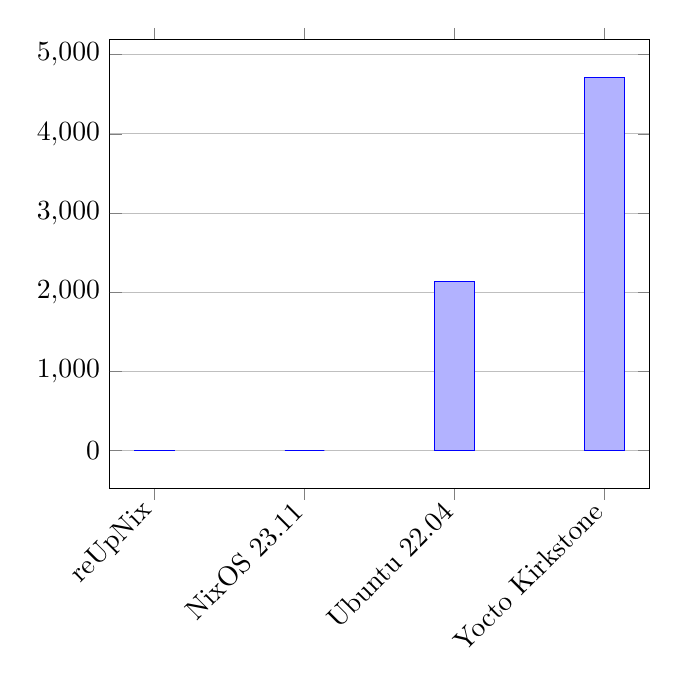
\begin{tikzpicture}
    \begin{axis}[
      ybar,
      bar width=0.5cm,
      % width=0.5\textwidth,
      % height=0.5\textwidth,
      xtick=data,
      xticklabels={
        {reUpNix},
        {NixOS 23.11},
        {Ubuntu 22.04},
        {Yocto Kirkstone}
      },
      x tick label style={rotate=45,anchor=east}, % Rotating labels
      ymajorgrids=true, % Major grid lines for y-axis
      ytick={0,1000,2000,3000,4000,5000}, % Y-axis tick marks
      extra y ticks={1000,2000,3000,4000}, % Additional y-axis tick marks
      extra y tick labels={}, % Remove labels for the extra ticks
      ]

      \addplot coordinates {
        (1,3.8)
        (2,0)
        (3,2134)
        (4,4717)
      };

    \end{axis}
  \end{tikzpicture}
\caption{Update Size by OS in Megabytes}
\end{figure}

\clearpage

\section{Time To Recover}
In order to verify that the \textit{reUpNix} system can recover from a reboot
in an acceptable time frame, we measured the time it takes for the system to
reboot and send a message via the \textit{Azure IoT Edge Hub} with the proposed
methodology from chapter \ref{sec:time-to-recover}. We used a sample application
to send the current timestamp to the \textit{Azure IoT Edge Hub} after the system
has rebooted. An excerpt from the sample application is shown in listing
\ref{lst:sampleapp}.


\begin{lstlisting}[
    caption={Sample App Which Sends The Current Timestamp Startup},
    label=lst:sampleapp]
namespace BA.SampleApp;

using System.Encoding;
using Microsoft.Azure.Devices.Client;

public class Program
{
  public static async Task Main(string[] args)
  {
    var currentTime = DateTime.UtcNow.ToString();
    var client = new DeviceClient.CreateFromEnvironment();
    var messageBytes = Encoding.UTF8.GetBytes(currentTime);
    var message = new Message(messageBytes);

    await client.SendEventAsync(message);
  }
}
\end{lstlisting}

\begin{table}[H]
	\centering
	\begin{tabular}{l|l|l|l}
	\toprule
		Operating System & Average & Std. Deviation & Std. Error \\
	\midrule
    \textbf{reUpNix} & 16.0 & 2.44 & 0.67 \\
    \textbf{NixOS 23.01} & 24.06 & 8.73 & 1.62 \\
    \textbf{Ubuntu 22.04} & 1.0 & 1.0 & 1.0 \\
    \textbf{Yocto Kirkstone} & 1.0 & 1.0 & 1.0 \\
	\bottomrule
	\end{tabular}
	\caption{Time to recover by OS in seconds}
	\label{tab:timetorecover}
\end{table}

\begin{figure}[H]
\centering
\begin{tikzpicture}
  \begin{axis}[
    title  = ReUpNix,
    ybar,
    bar width=0.15cm,
    enlarge y limits  = {0.15,upper},
    width = 0.5\textwidth,
  ]
    \addplot table [x=seconds, y=times, col sep=comma] {data/time-to-recover-reupnix.csv};
    \draw[dashed,red] (axis cs:15.33,\pgfkeysvalueof{/pgfplots/ymin}) -- (axis cs:15.33,\pgfkeysvalueof{/pgfplots/ymax});
    \draw[dashed] (axis cs:16,\pgfkeysvalueof{/pgfplots/ymin}) -- (axis cs:16,\pgfkeysvalueof{/pgfplots/ymax});
    \draw[dashed,red] (axis cs:16.67,\pgfkeysvalueof{/pgfplots/ymin}) -- (axis cs:16.67,\pgfkeysvalueof{/pgfplots/ymax});
  \end{axis}
\end{tikzpicture}
\begin{tikzpicture}
  \begin{axis}[
    title  = NixOS,
    ybar,
    bar width=0.15cm,
    enlarge y limits  = {0.15,upper},
    width = 0.5\textwidth,
    % nodes near coords,
  ]
    \addplot table [x=seconds, y=times, col sep=comma] {data/time-to-recover-nixos.csv};
    \draw[dashed,red] (axis cs:22.44,\pgfkeysvalueof{/pgfplots/ymin}) -- (axis cs:22.44,\pgfkeysvalueof{/pgfplots/ymax});
    \draw[dashed] (axis cs:24.06,\pgfkeysvalueof{/pgfplots/ymin}) -- (axis cs:24.06,\pgfkeysvalueof{/pgfplots/ymax});
    \draw[dashed,red] (axis cs:25.68,\pgfkeysvalueof{/pgfplots/ymin}) -- (axis cs:25.68,\pgfkeysvalueof{/pgfplots/ymax});
  \end{axis}
\end{tikzpicture}
\begin{tikzpicture}
  \begin{axis}[
    title  = Ubuntu 22.04,
    ybar,
    enlarge y limits  = {0.15,upper},
    width = 0.5\textwidth,
    nodes near coords,
  ]
    \addplot table [x=seconds, y=times, col sep=comma] {data/time-to-recover-ubuntu.csv};
  \end{axis}
\end{tikzpicture}
\begin{tikzpicture}
  \begin{axis}[
    title  = Yocto Kirkstone,
    ybar,
    enlarge y limits  = {0.15,upper},
    width = 0.5\textwidth,
    nodes near coords,
  ]
    \addplot table [x=seconds, y=times, col sep=comma] {data/time-to-recover-yocto.csv};
  \end{axis}
\end{tikzpicture}
\caption{Time of recovery after a reboot by OS in seconds.}
\end{figure}

\clearpage
\section{Container Updates}
With the proposed methodology in chapter \ref{sec:container-updates} we were able
to install \ac{OCI}-container images
on an \ac{IoT} device running \textit{reUpNix} without using \code{docker pull}.
We verified that the installed images can be used to run containers with \textit{Docker}
and match the images from \textit{Docker Hub} by comparing the \textit{SHA256} checksums.
Since the images are now stored in the \textit{Nix} store, we used the \textit{reUpNix}
differential update mechanism to install the container images and compared the update size
with the compressed size that would be downloaded with \code{docker pull}. We used
the same compression algorithm (\textit{gzip}) to compress the update artifacts,
as \textit{Docker} uses to compress the container images. With this methodology
we tested the top 10 most pulled images from \textit{Docker Hub} and the results
can be seen in table \ref{tab:container-size} and figure \ref{fig:container-size}.

\begin{figure}[htbp]
  \centering
  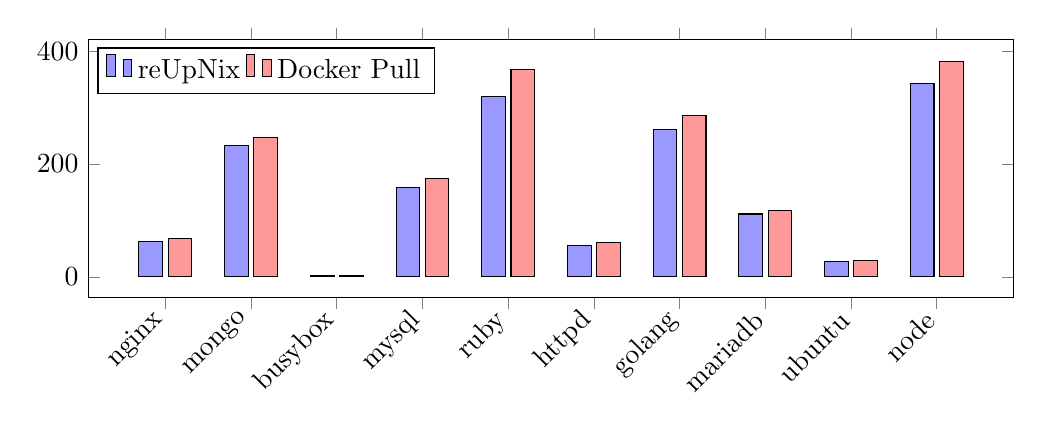
\begin{tikzpicture}
    \begin{axis}[
      ybar,
      bar width=0.5cm,
      width=1.1\textwidth,
      height=0.4\textwidth,
      bar width=0.3cm,
      xtick=data,
      xticklabels={
        nginx, mongo, busybox, mysql, ruby, httpd, golang, mariadb, ubuntu, node
      },
      x tick label style={rotate=45,anchor=east},
      legend style={
        at={(0.01,0.97)},
        anchor=north west,
        legend columns=-1,
      }
      ]

      \addplot[fill=blue!40] coordinates {
        (1,61.83) % nginx
        (2,233.22) % mongo
        (3,2.03) % busybox
        (4,158.14) % mysql
        (5,319.78) % ruby
        (6,55.22) % httpd
        (7,261.24)  % golang
        (8,111.46) % mariadb
        (9,26.38) % ubuntu
        (10,343.49) % node
      };

      \addplot[fill=red!40] coordinates {
        (1,67.25) % nginx
        (2,246.58 ) % mongo
        (3,2.05) % busybox
        (4,174.94 ) % mysql
        (5,367.45 ) % ruby
        (6,61.53 ) % httpd
        (7,285.59 ) % golang
        (8,117.04 ) % mariadb
        (9,28.17 ) % ubuntu
        (10,382.26 ) % node
      };

      \legend{reUpNix, Docker Pull}
    \end{axis}
  \end{tikzpicture}
  \caption{Container Image Download Size in MB}
  \label{fig:container-size}
\end{figure}

\clearpage

\begin{table}[H]
	\centering
	\begin{tabular}{l|l|l|l}
	\toprule
		Container Image & Docker Pull Size & reUpNix Size & $\Delta$ \% \\
	\midrule
    \textbf{nginx} & 67.25 MB & 61.83 MB & \color{ba-green}{- 8.0\%} \\
    \textbf{mongo} & 246.58 MB & 233.22 MB & \color{ba-green}{- 5.6\%} \\
    \textbf{busybox} & 2.05 MB & 2.03 MB & \color{ba-green}{- 0.9\%} \\
    \textbf{mysql} & 174.94 MB & 158.14 MB & \color{ba-green}{- 9.6\%} \\
    \textbf{ruby} & 367.45 MB & 319.78 MB & \color{ba-green}{- 12.9\%} \\
    \textbf{httpd} & 61.53 MB & 55.22 MB & \color{ba-green}{- 10.2\%} \\
    \textbf{golang} & 285.59 MB & 261.24 MB & \color{ba-green}{- 8.5\%} \\
    \textbf{mariadb} & 117.04 MB & 111.46 MB & \color{ba-green}{- 4.7\%} \\
    \textbf{ubuntu} & 28.17 MB & 26.38 MB & \color{ba-green}{- 6.3\%} \\
    \textbf{node} & 382.26 MB & 343.49 MB & \color{ba-green}{- 10.1\%} \\
	\bottomrule
	\end{tabular}
	\caption{Container Image Download Size}
	\label{tab:container-size}
\end{table}

\noindent
We can see from the results that the \textit{reUpNix} differential update mechanism
is more efficient in installing container image updates than using \code{docker pull}.
For all of the top 10 most pulled images from \textit{Docker Hub}, we can save
transferred data size by using \textit{reUpNix}. Even container images that are
only a few Megabytes in size, like \textit{busybox}, can be transmitted in a more
efficient way with \textit{reUpNix}'s differential update methodology. This means
that using \textit{reUpNix} to install container images on \ac{IoT} devices, is more
efficient than using \code{docker pull} and our proposed methodology can be used
as a replacement which still works with \textit{Azure IoT Edge}.

